%%%%%%%%%%%%%%
% To compile the latex source you the following packages
\documentclass[11pt,a4paper]{article}
\usepackage{color}
\usepackage{listings}
\usepackage{graphicx}
\usepackage{url}
\usepackage[ddmmyyyy]{datetime} 
\renewcommand{\dateseparator}{-}

\definecolor{bbb}{rgb}{.9,.9,.9}
\lstset{stepnumber=2, basicstyle=\small \ttfamily, language=matlab,
  frame=single, framerule=0.pt}

\usepackage[colorlinks=true, pdfstartview=FitV, linkcolor=blue,
citecolor=blue, urlcolor=blue]{hyperref}

\newcommand\kms{$\mathrm{km} \, \mathrm{s}^{-1}$}
\newcommand\kmsmath{\mathrm{km} \, \mathrm{s}^{-1}}



%%%%%%%%%%%%%%%%%%%%%%%%%%%%
%%%%%% Page dimensions %%%%%
%%%%%%  DO NOT CHANGE  %%%%%
%%%%%%%%%%%%%%%%%%%%%%%%%%%%

%\textheight=247mm
\textwidth=163mm
\topmargin=-7mm
\oddsidemargin=-10mm
\evensidemargin=-10mm
%\parindent 10pt

\setlength{\textwidth}{16.3cm}
\setlength{\oddsidemargin}{0cm}
\setlength{\evensidemargin}{0cm}
\addtolength{\textheight}{20mm}
\addtolength{\voffset}{-5mm}
\usepackage{sectsty}
\usepackage[small,bf,hang]{caption}

\allsectionsfont{\sffamily}
\chapterfont{\sffamily}
\chaptertitlefont{\sffamily}


%%%%%%%%%%%%%%%%%%%%%%%%%%%%%
%%%%% Start of document %%%%% 
%%%%%%%%%%%%%%%%%%%%%%%%%%%%%

\begin{document}
\pagestyle{plain}
\pagenumbering{arabic}
\title{\textsf{Analysing data from SALSA using \textsc{SalsaJ}}}
\author{\textsf{Eskil Varenius}}
\yyyymmdddate
\date{\textsf{Revised: \today \, \currenttime}}
 

\maketitle

\section*{Abstract}
This document describes how to analyse FITS files generated by the SALSA Onsala
radio telescopes by using the software \textsc{SalsaJ}.  We describe step by
step how will open the FITS files, improve the analysis by removing receiver
artifacts (spectral baseline subtraction), and fit Gaussian intensity
distributions to derive velocities and intensities for the observed components
(peaks).

\tableofcontents

\section{Introduction}
\label{sec:introduction}

The SALSA Onsala telescope is a 2.3\,m in diameter antenna located at
Onsala space observatory outside Gothenburg. The telescopes are
designed to detect the faint radiation from cold hydrogen gas in our
galaxy, the Milky way. The hydrogen gas emits radiation at a
wavelength of 21 cm (or a frequency of 1420.4 MHz). This signal can be
detected by the microwave receiver connected to the telescope. 
The observed spectrum can be
exported into a FITS-file, which is the currently most used type of
file for astronomical images and spectra. The fits file has two parts:
(1) a \emph{header} which includes information
about the data such as the velocity resolution, central frequency and
many others, and (2) the data itself.

Having completed the observations, the observer may want to process
the data further in order to more accurately deduce the kinematics,
as well as the amount of hydrogen gas in the Milky Way. There
are currently two main ways to analyse data from SALSA:

\begin{itemize}
\item \textbf{SalsaJ} was developed within the EU-HOU project.
	SalsaJ can be used to analyse spectral data from the SALSA telscopes, but
	can also be used as a simple image editor and processor.  The main
	advantage of SalsaJ is its easy-to-use point-and-click interface. The main
	disadvantage is that reducing many spectra can be tedious.
\item \textbf{SalsaSpectrum} is a data reduction environment written
  in the popular mathematical software \textsc{\textsc{Matlab}} -
  aimed for reduction of data from SALSA Onsala, developed by Daniel
  Dahlin. The main advantage is that many spectra can be processed
  quickly. The main disadvantage is that it requires the user to have
  a working installation of Matlab, which is non-free software. Please note 
  that the observatory cannot provide Matlab licenses, but many university
  students have free access to Matlab.
\end{itemize}
Both SalsaJ and SalsaSpectrum can be downloaded from the webpage at
{\url{http://vale.oso.chalmers.se/salsa}}. 

\section{Analysing SALSA data with SalsaJ}
\label{sec:salsaj}
In this section we describe step by step how to analyse the FITS files
generated by the SALSA Onsala telescopes in the software SalsaJ. We will
open the FITS files, switch to velocity, and inspect the data using the
pointer. Further analysis, such as removing receiver artifacts 
(spectral baseline subtraction), and fit Gaussian intensity distributions,
is described in Sect. \ref{sect:adv}.
\textbf{IMPORTANT:} SalsaJ can only read correctly spectra produced by SALSA after
2015-06-23.  If you have older spectra, you cannot use SalsaJ for processing
them.

\subsection{Starting SalsaJ}
Once you have downloaded the file SalsaJ2.jar from the website, 
open it by double clicking. If this does not work for you, 
try right-clicking on the file SalsaJ2.jar and chose \emph{Open with}
and find \emph{Java}. Once the software open you should see a window looking
like Fig. \ref{fig:salsajstart}.
\begin{figure}[h!]
  \centering
  \scalebox{0.55}{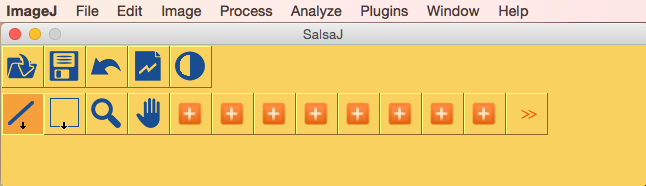
\includegraphics{../figures/start}}
  \caption{The startup window of the software SalsaJ.}
  \label{fig:salsajstart}
\end{figure}

\subsection{Opening a spectrum}
To open a spectrum, i.e. a FITS file, click the \emph{File} menu, and then
\emph{Radio spectrum}. Navigate to the file you want to analyse and click OK.
You should now see the spectrum presented as a figure similar to Fig. 
\ref{fig:opened}.
\begin{figure}[h!]
  \centering
  \scalebox{0.55}{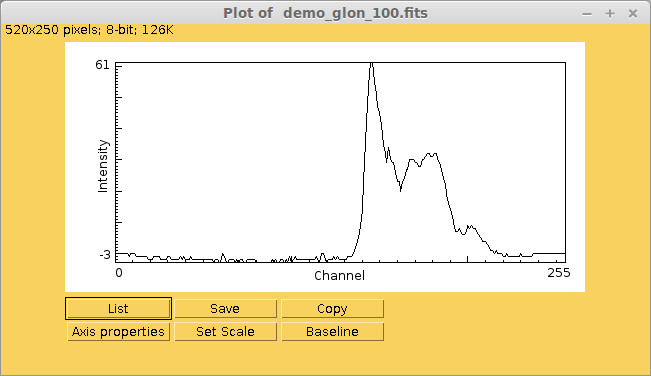
\includegraphics{../figures/spectrumopened}}
  \caption{A spectrum has been opened and is by default presented with channel
  index on the horisontal axis. We want to change to velocity.}
  \label{fig:opened}
\end{figure}
Note: If you in Mac OS X do not see the \emph{Radio spectrum} option in the
\emph{File} menu, make sure you focus the SalsaJ window by clicking on it.

\subsection{Set the scale}
By default, SalsaJ presents spectra as Intensity vs channel number. For our
purposes it is more useful to switch the horisontal axis to velocity. This is
done by clicking the button labelled \emph{Set scale}, choose \emph{Velocity},
and click OK. The horisontal axis should now be set to km/s, as in Fig.
\ref{fig:velocity}. Note that you can inspect the measured values by moving the
pointer over the graph: the intensity and velocity are reported in the lower part
of the window. If you are only interested in rough estimates of velocities,
you can note down the values you find by visual inspection and consider yourself finished
with this spectrum. However, if you want to get the best possible results you may 
want to consider the baseline subtraction and gaussian fitting described in Sect. 
\ref{sect:adv} below.
\begin{figure}[h!]
  \centering
  \scalebox{0.55}{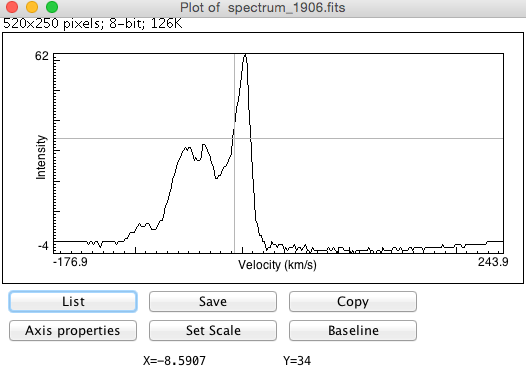
\includegraphics{../figures/spectrumvel}}
  \caption{The spectrum is now shown with velocity on the horisontal axis. You can now
  inspect the spectrum directly by hovering with the pointer over the peaks. The current value
  marked by the cross is displayed in the bottom part of the window.}
  \label{fig:velocity}
\end{figure}

\section{Advanced processing}
\label{sect:adv}
You can get pretty good estimates of the observed velocities by moving the
pointer over the graph: the intensity and velocity are reported in the lower
part of the window.  However, if you want to get the best possible results you
may want to consider the baseline subtraction and gaussian fitting as described
below.  Note that this can be tedious work if you have many spectra, in this
case consider using the Matlab program SalsaSpectrum if you have access to
Matlab.

\subsection{Spectral baseline subtraction}
The spectra presented in Fig. \ref{fig:velocity} is pretty good already from 
the start, but looking carefully we can see that the zero-level is not flat. 
Instead, it is curved due to residual effects from the receiver which were
not subtracted during the observation. 
For accurate results, we need to 
remove this effect. This removal is called \emph{baseline subtraction} and 
is started by clicking the button \emph{Baseline} in the SalsaJ window.
From quickly inspecting the graph 
with the pointer, we note that we have no line emission in the velocity regions
[-170 to -130] and [50 to 240] km/s. 
We enter the boundaries of the two regions and chose poynomial order 2, 
see Fig. \ref{fig:baseline}.

\begin{figure}[h!]
  \centering
  \scalebox{0.55}{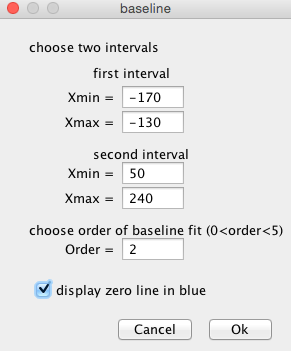
\includegraphics{../figures/baseline}}
  \caption{The input window for baseline subtraction, where we have defined
  two regions of the spectra with no line emission and chosen a degree of 
  polynomial to fit to the data.}
  \label{fig:baseline}
\end{figure}

After you press OK, a baseline will be fitted and plotted, see Fig. 
\ref{fig:baselinefit}.
\begin{figure}[h!]
  \centering
  \scalebox{0.55}{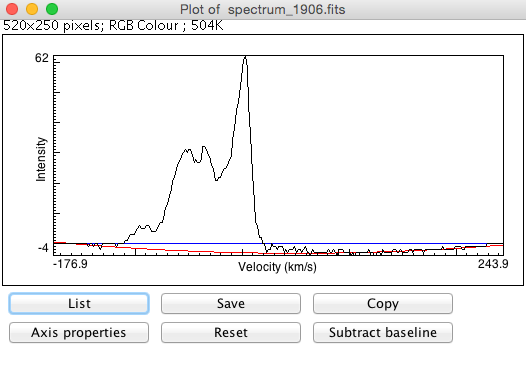
\includegraphics{../figures/baselinefitted}}
  \caption{A baseline has been fitted based on the input in Fig. 
  \ref{fig:baseline}. The fitted baseline is shown in red, and the 
  zero-level in blue.}
  \label{fig:baselinefit}
\end{figure}
If you are happy with the fit, click \emph{Subtract baseline}. If the fit looks
bad, click \emph{reset} and redo the subtraction with different intervals or
polynomial orders until you get a good fit to the line-free parts of the spectrum.
After subtracting a baseline, the line-free parts should be flat, as in 
Fig. \ref{fig:baselinesubtracted}.
\begin{figure}[h!]
  \centering
  \scalebox{0.55}{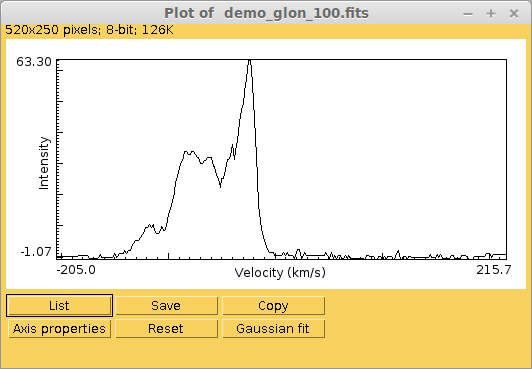
\includegraphics{../figures/baselinesubtracted}}
  \caption{The baseline fitted in Fig. \ref{fig:baselinesubtracted} has been
	  subtracted and the line-free regions are flat with noise around zero. We are now
	  ready to measure velocities and intensities.}
  \label{fig:baselinesubtracted}
\end{figure}

\subsection{Measuring velocities: fitting Gaussians}
Because of noise it can be hard to measure exactly the center velocity
of peaks by simple manual inspection. A good way is to fit Gaussian
intensity distributions to the peak, which can be done by clicking the
button \emph{Gaussian fit} in SalsaJ. For the fitting we first need to
note down starting guesses for the peaks we want to fit. Here visual
inspection suggest four peaks roughly at positions -90, -52, -35, and 0 km/s. 
Hence we want to fit four Gaussians to the spectrum, but SalsaJ can only
handle one at the time (the SalsaSpectrum Matlab class can fit multiple Gaussians 
at once). Let us start with the brightest peak around 0 km/s. 

After clicking the button\emph{Gaussian fit} we need to give an interval of data to use
for fitting this peak, specified by Xmin and Xmax. Usually a range of 10km/s above and below the
peak center works fine, in this case -10 to +10. Then we need to give initial guesses for the fitting
to start. This does not have to be very accurate, but the closer to the real value the better.
We guess an amplitude of 30 (which is far below the real one), a center at 0 as noted for the 
peak positions in the previous paragraph, and a width of 20. Then we click OK. The fitted Gaussian
is shown in red, see Fig. \ref{fig:fittedgaussian}. 

NOTE: If your fit goes wrong, for example
if you specify an interval of the data where there is no peak, then you can remove the previous fitted
gaussian by checking the box \emph{erase the last}. 

We proceed in a similar way to fit the other three peaks, the result can be seen in Fig. 
\ref{fig:allfitted}. After fitting you will also get a list of fitted values, see Fig. 
\ref{fig:fitres}. From this list you can read the galactic coordinates of the spectrum, 
and the velocities and intensities of the all fitted peaks. The velocities can be used
to make a rotation curve or map of the Milky Way as described in the SALSA Milky Way project 
instructions.


\begin{figure}[h!]
  \centering
  \scalebox{0.55}{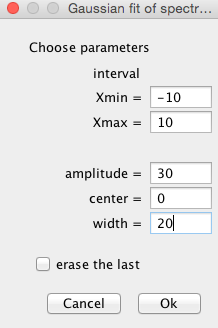
\includegraphics{../figures/fitpars}}
  \caption{A set of parameters to fit a Gaussian intensity distribution to 
	  one of the peaks in the spectrum. The resulting fit can be seen in Fig. 
  \ref{fig:fittedgaussian}.} \label{fig:fitpars}
\end{figure}

\begin{figure}[h!]
  \centering
  \scalebox{0.55}{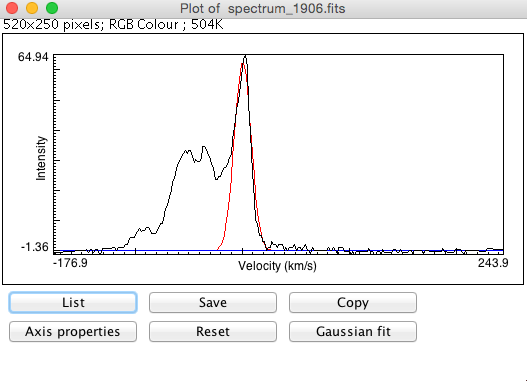
\includegraphics{../figures/fittedgauss}}
  \caption{A gaussian has been fitted to the data using the parameters
  specified in Fig. \ref{fig:fitpars}.} \label{fig:fittedgaussian}
\end{figure}

\begin{figure}[h!]
  \centering
  \scalebox{0.55}{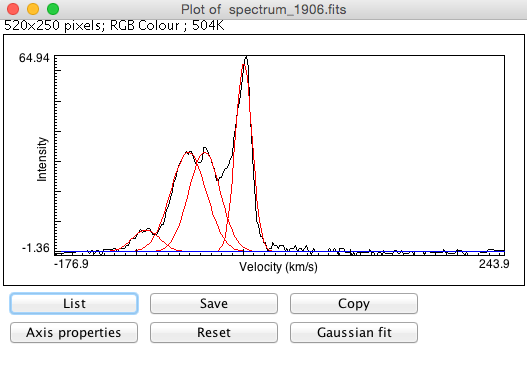
\includegraphics{../figures/allfitted}}
  \caption{All four peaks have been fitted. The fitted velocities and intensities can be
	  found in the \emph{Gaussian fit results}, see Fig. \ref{fig:fitres}.} \label{fig:allfitted}
\end{figure}

\begin{figure}[h!]
  \centering
  \scalebox{0.55}{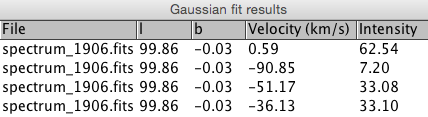
\includegraphics{../figures/fitres}}
  \caption{All four peaks have been fitted. In this window you can read the fitted velocities and 
	  intensities. These values can be used to make a rotation curve or map of the Milky Way, as 
  described in the SALSA project instructions document.} \label{fig:fitres}
\end{figure}


\end{document}

